\documentclass[a4paper, 11pt]{article}

\usepackage{natbib}
\bibliographystyle{agsm}
\setcitestyle{authoryear,open={(},close={)}}

\usepackage{fontspec}
\setmainfont[Ligatures=TeX]{Lato Light}

\usepackage{graphicx}
\usepackage{wrapfig}

\linespread{1.05}

\makeatletter
\renewcommand{\maketitle}{
\begin{flushright}
{\LARGE\@title}

\vspace{50pt}

{\large\@author}
\\\@date 
\vspace{40pt}
\end{flushright}
}
\renewcommand{\@seccntformat}[1]{}
\makeatother


\title{\textbf{The impact of digital Media on Design}\\Media Facades}

\author{\textsc{Ans Vaessen}
\\{\textit{13009722}}}

\date{\today\\ \ \\
word count: 2..}

%%%%%%%%%%%%%%%%% START %%%%%%%%%%%%%%%%%%

\begin{document}
\maketitle

\begin{abstract}
This essay examines The impact of digital media on the urban space by looking at the buidling facades and the use of newe media. 
in particular 
and also 
change over the years from one way  communication to both ways....

\end{abstract}

\vspace{30pt} % Some vertical space between the abstract and first section

\section*{Introduction}
Public space ?
NEw media

Even if they are private buildings they are in the public sphere and impacting it.

Urban media with a couple of exampes

One buidling with a very famous facade is Picadilly Circus. Famous for being one of te first to have light advertisement. But also a good example of how facades change and influence the public space. Also with the developemnt of new media the advertisement in Picadily circus changed as well. 

It is this facade and the different content it is showing that is used as the main exmaple of how digital media impact design.  Or do I want to use kinetic facades as well....

\section{Literature review give it a tittle!}

\subsection{urban space and media facades}
Urban space 
some literature 


\subsection{genres}
\cite{fritsch2008a} states that Architecture has always been changing and renewing itself by using new ways, materials or in this case media. There are a number of genres introduced by \cite{fritsch2008a} see also figure ...
Advertising is named as an archetype example. But also News like ont he Reuters Building. 


Figure \ref{fig:graph1} illustrates how this works. The big company is sustaining the technology or innovation and performs better over time. So much so that they leave the mainstream and move into the high end market. At the same time the new entrant is improving its product and enters the mainstream in time to take over from the incumbent \citep{Christensen97}.

\begin{figure}[h!]
    \centering
    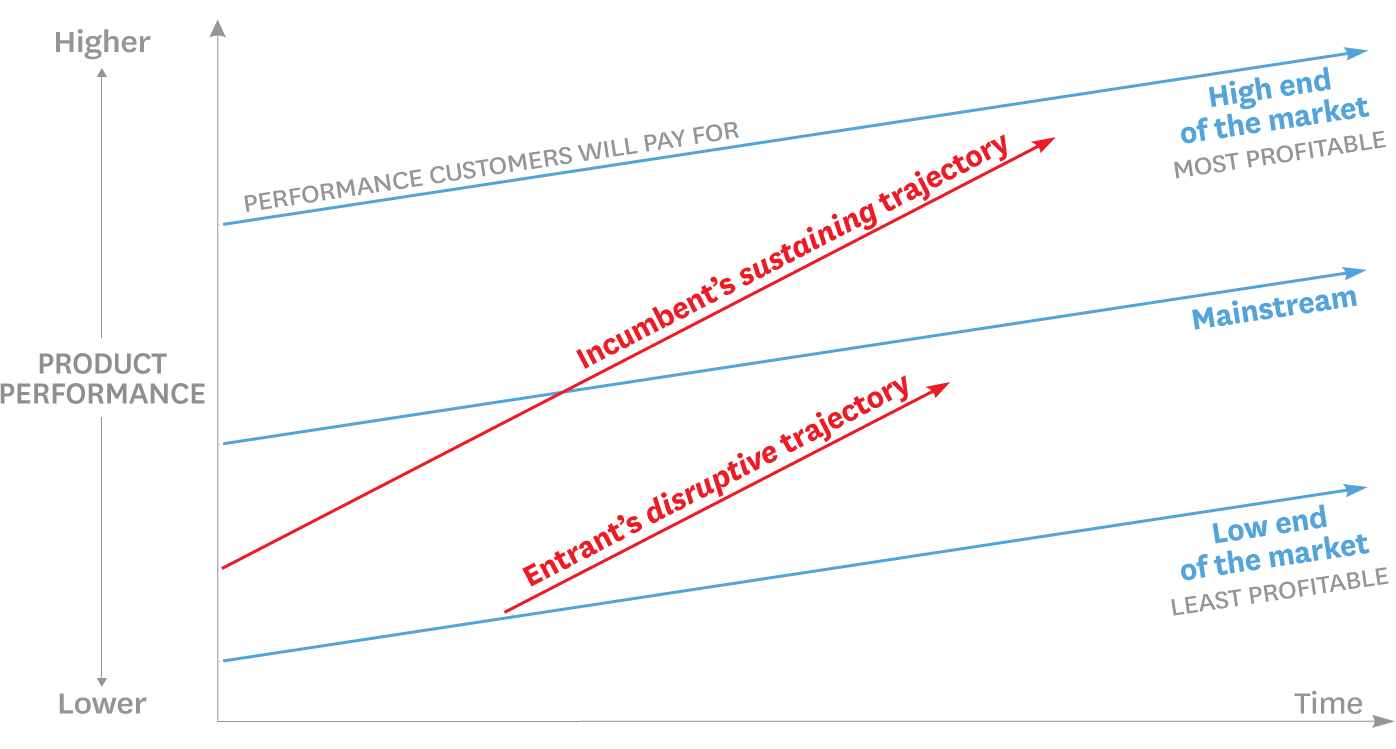
\includegraphics[width=0.9\textwidth]{big-model.png}
    \caption{Model of disruptive innovation \citep{Christensen2015}.}
    \label{fig:graph1}
\end{figure}


\subsection{The impact environment, content, context}

\cite{Daalsgaard2010} looks at the place, whats on the screen and how this can influence


\subsection{content and social media}

How facades can use social media

\subsection{content mirror or window}

If content isn't working how does tis influence the preception. is it just a window or even worse you don't even notice it at all. What will make you look.

\subsection{use of date}

Kinetcic facades using weather/ temperature and light as input to change the facade.
But also smart data face or brand recognition and advertisments pushed not only online but also in real life when walking he streets.


\section{Piccadilly Circus}

The advertisment on Picadilly is more than 100 years old. an overview in the \cite{telegraph2011} shows the first illuminated advertisements dates back to 1908. Later \cite{nelson_1998} writes how The lights are moving with time and switching to digital billboards. Managing Director of the design house Sedley Place Mick Nash is cited in the article saying: "It blends art, science and commerce. We have called it Street Vision because it is a whole new way of talking to the public. It is not TV and not a poster, but a new type of media which cuts across those two."\cite{nelson1998}.

But even more recent the Bill Boards have become interactive the next examples will be examined using the literature frameworks discussed in (refer to former chapter) 

\subsection{Content, environment context}

Mostly ads but also to commemarate WW1


\subsection{social media}

used to ineract via social media MAC donals twice


first with making pictures


later with making avatars


\subsection{use of date}


Looking at the cars the brand and commercia reflecting the type of people

ALso interface..

Mischien kort iets doen met de 



\section{critcal reflection}
\label{reaction}


ethical using data 

URban space
boredom no seeing it anymore





\section{Conclusion}




\cite{Diaconu}, recommends Ryanair to start flying from the main airports to get hold of more travellers and business travellers in particular. In their report \cite{Eurocontrol2018} describes how low cost carriers attempt to penetrate the long haul market. If Ryanair succeeds in these and other changes they would fit the model better. But as \cite{Christensen2015} warns the main airlines might be creative and out smart the low cost carriers like Ryanair.




%% disable some things
\renewcommand{\textbf}{}
\renewcommand{\bf}{}
\bibliography{biblio}{}
\end{document}
